\section{Vorbetrachtung und Verwandte Arbeiten}
\label{sec:relatedwork}

Als erstes gilt es, gegenwärtige Technologien zu evaluieren, um eine solide Grundlage für eine verteilte Dateiverwaltung für die Schul-Cloud zu erstellen. Wie in der Einleitung erwähnt wurde, soll kein neuartiges Dateiverwaltungskonzept geschaffen werden. Vielmehr soll auf bestehenden Systemen und Technologien aufgebaut werden und deren Vorteile genutzt werden. Zu Beginn werden im Vorfeld formulierte Anforderungen aufgegriffen und analysiert. Hierzu diente der Technischen Bericht der Schul-Cloud \cite{paper:technischerbericht} als Grundlage, welcher in Zusammenarbeit des Hasso-Plattner-Instut mit dem Mint-EC enstand. Ebenfalls werden andere Konzepte zur Dateiverwaltung im Schul-Kontext durchsichtet und analysiert. Es schließt sich eine Beobachtung an, inwieweit Dateiablagen auf Basis von Cloud-Storage Provider bereits im Unterricht genutzt werden. Für eine abschließende Vorbetrachtung eignet sich eine Betrachtung bereits bestehender Cloud-Storage Anbieter, welche sich in der Praxis bewährt haben und weiträumigen Einsatz finden.

\subsection{Anforderungen an die Schul-Cloud}

\begin{center}
	
	\begin{figure}[H]
		\begin{center}
			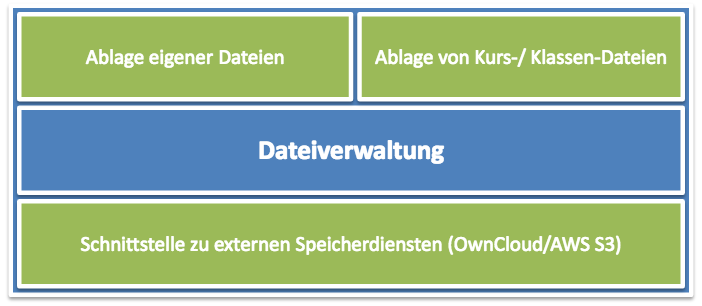
\includegraphics[width=0.8\linewidth]{images/AnforderungenDateiverwaltung}
			\caption[Caption for relatedWork]{Grundanforderungen an die Dateiverwaltung der Schul-Cloud\footnotemark}
			\label{fig:devices}
		\end{center}
	\end{figure}
	\footnotetext{Martin Hense (Mint-EC - \url{https://www.mint-ec.de/})}
\end{center}

\todo[inline]{andere Studien, Nutzung bei Hausaufgaben (https://www.bitkom.org/noindex/Publikationen/2010/Studie/Studie-Bildung-2-0-Digitale-Medien-in-Schulen/BITKOM-Studie-Bildung-20.pdf)}

\subsection{Nutzung von Cloud-Storage Provider im Unterricht}


Die Verwaltung von eigenen und geteilten Dateien wird mit der zunehmenden Digitalisierung des Unterrichts immer wichtiger. Wo es früher reichte, seine Unterrichtsmaterialien in einem Schulhefter zu legen, will man Arbeitsblätter und Wissenstexte heute überall und immer verfügbar haben. Um einen Eindruck in diese Problematik zu bekommen, wurde eine Umfrage zum Thema 'Dateiorganisation in der Schule' \cite{survey:umfragedateiorganisation} erstellt und an ehemaligen und aktuellen Schülern sowie Lehrern geschickt. Insgesamt nahmen \textbf{\textit{65}} \todo{Anpassen} Teilnehmer  an dieser Umfrage teil. Gefragt wurde unter anderem nach der Rolle des Teilnehmers (Schüler oder Lehrer) gefragt (Frage 1). Dabei sollten ehemalige Schüler und Lehrer vergangene Erfahrungen in die Beantwortung der Frage einfließen lassen. Dann wurde danach gefragt, ob der Befragte webbasierte Anwendungen zur Verwaltung der Dateien im Schulalltag benutzt hat (Frage 2). Anschließend wurde die Befragung geteilt. Wenn die Frage 2 mit 'Nein' beantwortet wurde, wurde nach Gründen für das Nichtbenutzen gefragt ()Frage 3). Wurde Frage 2 mit 'Ja' beantwortet, wurde nach Vorteilen der Nutzung gefragt (Frage 4), sowie nach Beispielen, welche Dienste genutzt wurden (Frage 5). 

Die Ergebnisse \cite{survey:umfragedateiorganisationergebnisse} dieser Umfrage zeigen, dass eine Mehrheit der Befragten (ca. 72\%) auf solche Anbieter in ihrem Schullaltag verzichtet haben. Ein Großteil dieser Mehrheit gab an, dass Datenschutz ein großes Problem dabei darstellte. Ausländische Anbieter wie Dropbox \footnote{Dropbox - \url{https://www.dropbox.com/de/?landing=cntl}} oder Google Drive \footnote{Google Drive - \url{https://www.google.com/intl/de_ALL/drive/}} werden im pädagogischen Bereich eher kritisch betrachtet, da sie nicht in Deutschland gehostet werden und somit keine Transparenz in der Weiternutzung anfallender Daten erfolgt. Auch sind solche Dienste in Lernplattformen eher verpönt, da ``Schulen keinen Einfluss auf die Verwendung und Weiternutzung der hier anfallenden Daten und haben keine Vertragsbeziehung mit dem Betreiber dieser Dienste" \cite{online:itslearningmythenundfakten} haben. Weitere Gründe für die Nichtnutzung sind unter anderem, dass weite Teile des Unterrichtsmaterials offline zur Verfügung stehen, wie zum Beispiel einfache Arbeitsblätter, welche gar nicht erst digitalisiert werden. Oft ist auch einfach die Bereitschaft auf Seiten von Lehrer und Schüler gar nicht vorhanden, ihre Dateien online verfügbar zu machen, da die Ausstattung an den Schulen ohnehin auf einen weniger digitalen Unterricht ausgerichtet ist. Dazu kommen veraltete Technologien und schnelles Internet. Somit besteht auch kein Interesse daran, diese Dateien nur für den Gebrauch zu Hause verfügbar zu machen. Wenn dann doch Dateien von zu Hause in die Schule gebracht werden müssen, zum Beispiel Präsentationen oder Videos, wurden diese einfach auf einem USB-Stick gelagert.

Ein kleiner Teil der Befragten (ca. 28 \%) nutzten oder nutzen dagegen bereits Cloud-Storage Dienste für ihre Dateiverwaltung. Als meistgenutzter Dienst wurden hier Google Drive, One Drive  \footnote{One Drive - \url{https://onedrive.live.com/}} und Dropbox genannt. Ein sehr kleiner Teil benutzte sogar selbstgehostete Dienste wie zum Beispiel eine ownCloud \footnote{ownCloud - \url{https://owncloud.org/}}. Die Gründe hierfür seien die stetige Verfügbarkeit von mehreren Geräten, die papierlose Nutzung von Unterrichtsmaterialien, ein leichterer Backup von wichtigen Dateien und das Teilen mit mehren Personen. 

Die Auswertung der Umfrage zeigt, dass bei einem Großteil die Nutzung von cloudbasierten File-Storage Diensten eher auf Kritik stößt, als sie wirklich genutzt werden. Vor allem sind Datenschutz und schlechter Umgang mit digitalen Medien im Unterricht die Gründe hierfür. Mit einer einfachen Lösung innerhalb der Schul-Cloud, schnell an nötige Dateien für den Unterricht oder Hausaufgaben in digitaler Form zu kommen, könnte man hier ein Umdenken umleiten und die Vorteile sichtbar machen.

\subsection{Bestehende Cloud-Storage Provider}

\todo[inline]{Todo: AWS S3 OwnCloud}

\clearpage
